% latex 论文样式
\documentclass{ctexart}

% 使用超链接宏包
\usepackage{hyperref}
% 设置纸张的宏包
\usepackage{geometry}
% 用户设置字体的宏包
\usepackage{fontspec}
\usepackage[fontsize=12pt]{fontsize}
% 文档标题宏包
\usepackage{titling}

% 覆盖 \maketitle 的相关指令,达到首页标题居中的目的
\renewcommand\maketitlehooka{\null\mbox{}\vfill}
\renewcommand\maketitlehookd{\vfill\null}

% 定义纸张大小为 A4,内容所占区域为 95%
\geometry{a4paper, scale=0.95}
% 定义超链接样式
\hypersetup{
	CJKbookmarks=true, % 支持中文书签
	colorlinks=true,
	citecolor=black,
	linkcolor=black,
	urlcolor=black,
	breaklinks=true % 允许链接中的换行
}

% 设置字体
% 设置英文字体
\setmainfont{JBHGXK}
% 设置中文字体
\setCJKmainfont{JBHGXK}

%作者
\author{aszswaz}


% 用于绘图的宏包
\usepackage{tikz}
% 用于书写数学公式的宏包
\usepackage{amsmath}

% 导入宏包
\usepackage{pgfplots}

% 一些包有多个模块,加载指定模块
\usetikzlibrary{positioning}

% 文档标题
\title{人工智能-基础篇}
\date{2022-03-17}

\begin{document}
\maketitle\newpage
\tableofcontents\newpage

\section{Rosenblatt 感知器}
\subsection{最基本的 Rosenblatt 感知器}
Rosenblatt 感知器是第一个从算法上完整描述的神经网络,它向人们展示了计算机对函数的自适应调整的可能性。

假设坐标系中存在一个端点 $(x_1, y_1)$,求一条从坐标轴原点出发,经过该端点的一条直线,过程如下:

设 $w$ 为直线的斜率、$e$ 为误差、$a$ 为学习率($0 \le a \le 1$),计算流程流程如下:

% 绘制 Rosenblatt 流程图
\begin{center}
	\begin{tikzpicture}[
			% 有圆角的长方形
			squarednode/.style={rectangle, draw=black, minimum size=5mm, rounded corners},
			% 看不见的像素点,用来连接线,达到折线的效果
			point/.style={coordinate, on grid}
		]
		\node[squarednode]      (maintopic)                                                 {输入$x_1$};
		\node[squarednode]      (gety)          [below of=maintopic]                        {$y = w \cdot x_1$};
		\node[squarednode]      (error)         [below of=gety]                             {$y_1 - y = e$};
		%Nodes
		\node[squarednode]      (neww)          [below of=error]                            {$n = w + a \cdot e \cdot x_1$};
		\node[squarednode]      (assgin)        [below of=neww]                             {$w = n$};
		\node[point]            (point1)        [left of=assgin, node distance=2cm]         {point1};

		%Lines
		\draw[->] (maintopic)       --            (gety);
		\draw[->] (gety)            --            (error);
		\draw[->] (error)           --            (neww);
		\draw[->] (neww)            --            (assgin);
		% 绘画一个点,并链接两条线,形成一个折线
		\draw[-]  (assgin)          --            (point1);
		\draw[->] (point1)          |-            (gety);
	\end{tikzpicture}
\end{center}
\url{rosenblatt.py}

Rosenblatt 感知器中,误差 $e$ 的计算公式为 $e = x^2w^2 - 2xyw + y^2$,在坐标系中,它是一个开口向上的抛物线:$y = ax^2 + bx + c$。

假设坐标系中,存在一个点:$x = 0.4, y = 0.68$,预测误差 $e$ 与斜率 $w$ 的关系为:

\[
	\begin{aligned}
		e & = 0.4^2 \times w^2 - 2 \times 0.4 \times 0.68 \times w + 0.68^2 \\
		  & = 0.16w^2 - 0.544w + 0.4624
	\end{aligned}
\]

% 绘制函数的抛物线
\begin{center}
	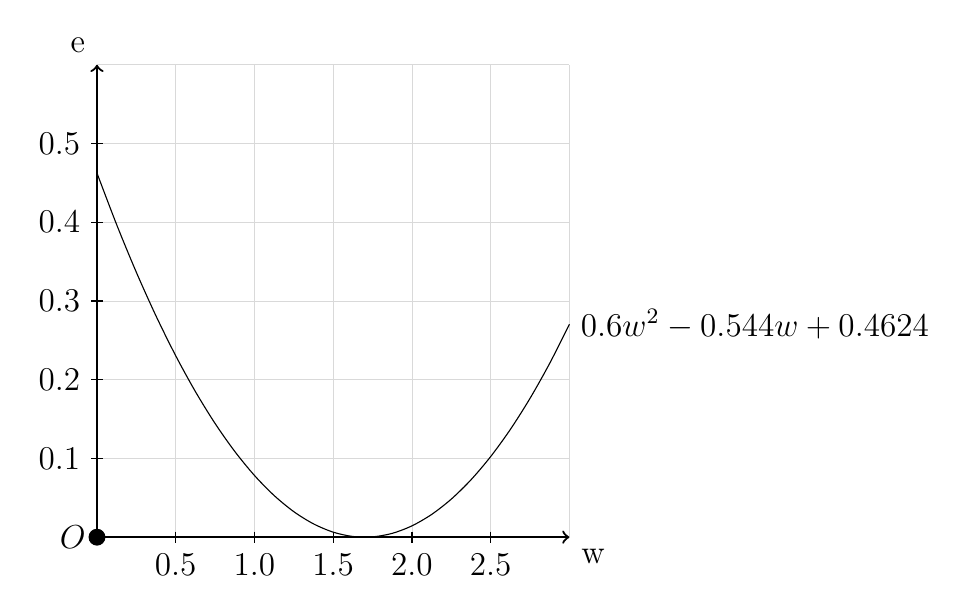
\begin{tikzpicture}
		% 绘制一个大小为 5 * 5 网格线
		\draw[help lines, color=gray!30] (0, 0) grid (6 cm, 6 cm);
		% 坐标轴原点
		\draw[fill] (0, 0) node [left]{$O$} circle(.1);
		% 绘制 y 轴和 x 轴
		\draw[thick, ->] (0, 0) -- (6 cm, 0) node[anchor = north west] {w};
		\draw[thick, ->] (0, 0) -- (0, 6 cm) node[anchor = south east] {e};

		% 画 X 轴和 y 轴的刻度
		\foreach \i/\x/\y in {1/0.5/0.1, 2/1.0/0.2, 3/1.5/0.3, 4/2.0/0.4, 5/2.5/0.5} {
				% 这里是用一个短短的直线表示刻度的点
				\draw (\i, 2pt) -- (\i, -2pt) node[anchor = north] {\x};
				\draw (2pt, \i) -- (-2pt, \i) node[anchor = east] {\y};
			}

		% 绘制函数在坐标轴上的抛物线
		\draw[color=black, smooth, domain=0:6] plot (\x, {(0.16 * (\x / 2)^2 - 0.544 * (\x / 2) + 0.4624) * 10}) node [right] {$0.6w^2 - 0.544w + 0.4624$};
	\end{tikzpicture}
\end{center}

如果存在多个点,预测误差的计算公式为:

\[
	\begin{aligned}
		e = \frac{1}{m} \sum^{m}_{i = 0} (x_1^2 \cdot w^2 - 2x_1 \cdot y_1 \cdot w + y_1^2)
	\end{aligned}
\]

此时这个 e 取得是所有的预测误差之和的平均数,所以它称为均方误差。

因为该函数满足一元二次函数:$y = ax^2 + bx + c$,所以它可以通过一元二次函数的求对称轴公式:$y = -\frac{b}{2a}$ 获得抛物线的最顶点:

首先,先转化为一元二次函数形式:

\[
	\begin{aligned}
		e & = \frac{1}{m} \sum^{m}_{i = 0} (x_1^2 \cdot w^2 - 2x_1 \cdot y_1 \cdot w + y_1^2)                                     \\
		  & = \frac{1}{m} \sum^{m}_{i = 0} x_1^2 \times w^2 - \frac{1}{m} \sum^{m}_{i = 0} w + \frac{1}{m} \sum^{m}_{i = 0} y_1^2
	\end{aligned}
\]

带入 $y = -\frac{b}{2a}$:

\[
	\begin{aligned}
		w & = \frac {
			\frac{1}{m} \sum\limits^{m}_{i = 0} (-2x_1y_1)
		}{
			2\frac{1}{m} \sum\limits^{m}_{i = 0} x_1^2
		}             \\
		  & = \frac {
			\sum\limits^{m}_{i = 0} (x_1y_1)
		} {
			\sum\limits^{m}_{i = 0} x_1^2
		}
	\end{aligned}
\]

这种一次性求出让误差最小的 w 取值的方法,也就是所谓的\textbf{正规方程}。

\url{variance-cost-function.py}

\end{document}
